\documentclass[a4paper]{article}
%\usepackage{exercise}
%um nur aufgaben zu zeigen
\usepackage[noanswer]{exercise} 
\usepackage{../task/images/preamble}
\usepackage{rotating}
\usetikzlibrary{decorations.pathmorphing}
\usetikzlibrary{decorations.markings}
\usetikzlibrary{arrows}
\usetikzlibrary{shapes.geometric}
\newcommand{\midarrow}{\tikz \draw[-triangle 90] (0,0) -- +(.02,0);}
\usepackage{xcolor}
%\usepackage{draftwatermark}
%\SetWatermarkText{\textsc{Draft 2}}
%\SetWatermarkScale{3}
%\SetWatermarkColor{red!30}

\usepackage[printwatermark]{xwatermark}
%\newsavebox\mybox
%\savebox\mybox{\tikz[color=red,opacity=0.3]\node{\textsc{Entwurf}};}
%\newwatermark*[
%allpages,
%angle=45,
%scale=10,
%xpos=-4cm,
%ypos=4cm
%]{\usebox\mybox}
\pagestyle{fancy}
\fancyhead[L]{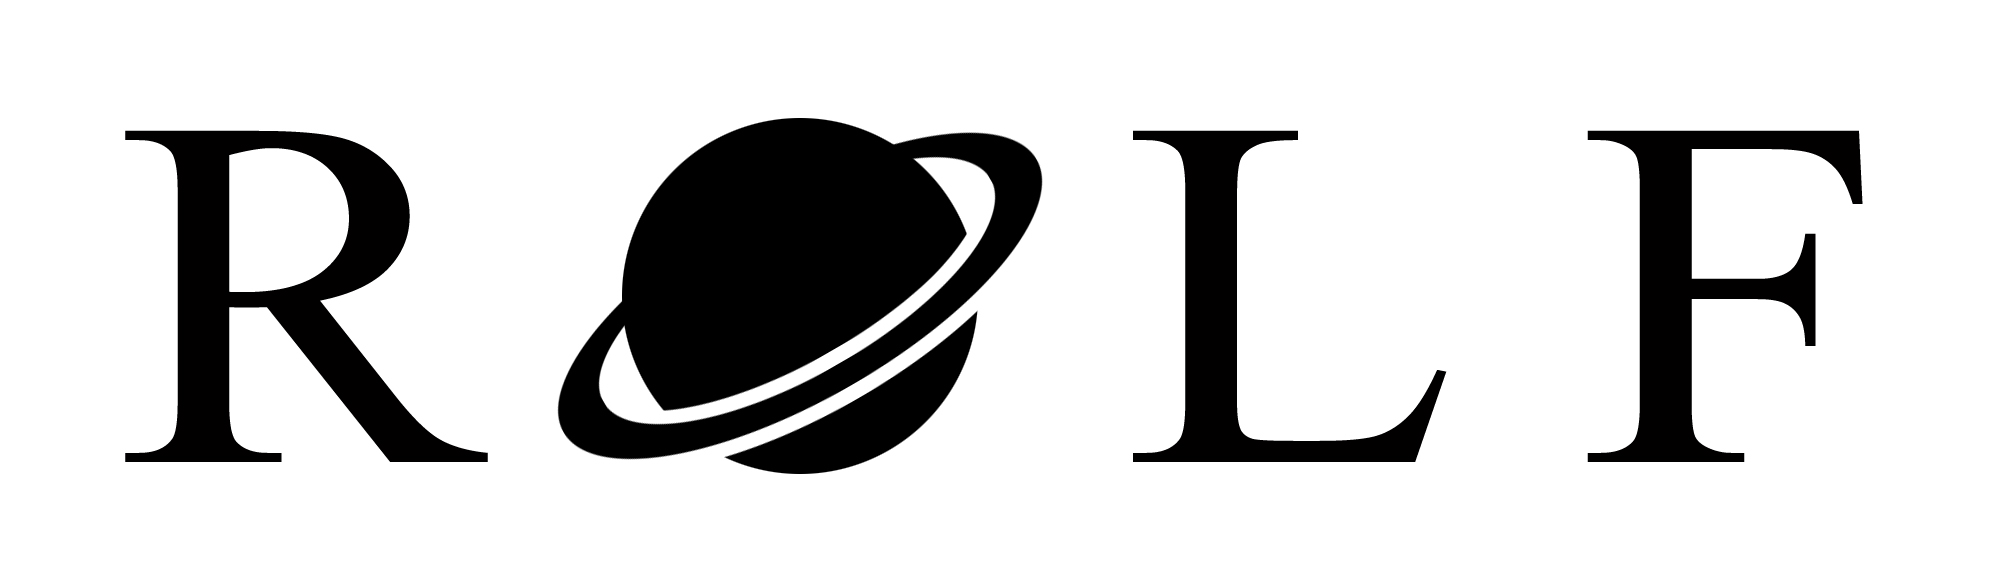
\includegraphics[width=2cm]{../images/rolfal.jpg}}
\fancyhead[R]{\textsc{Lösung Aufgabenserie 4}}


\begin{document}
	\vspace*{-1cm}
	\parbox{4cm}{\vspace{-0.2cm}
\includegraphics[width=5cm]{../task/images/logo_scaled.pdf}}
	\parbox{12.5cm}{\setstretch{2.0} \centering{ \Huge \textsf{ROLF stellt sich vor 
			}}}\\
			%Abgabe: 5. Oktober \\ \vspace*{-.5cm} }
		\vspace{0.5cm}

\thispagestyle{empty}


\noindent

\section*{Wer wir sind}
ROLF, der Rat der Oberstufe zum Lernen und Forschen, ist eine Gruppe von Oberstufenschülern und Studenten, die Spaß an Physik und vor allem auch an Physikwettbewerben haben.

\section*{Was wir wollen}
ROLF möchte interessierte Schüler dabei unterstützen, sich in ihrer Freizeit mit Physik zu beschäftigen. Dazu gehört für uns auch, aber selbstverständlich nicht nur, die Vorbereitung auf und die Teilnahme an Wettbewerben. In unserer Erfahrung stellen sie nämlich eine großartige Möglichkeit dar, sich mit der Physik auseinanderzusetzen. Natürlich lernt man bei Wettbewerben sehr viel, aber was vielleicht noch wichtiger ist: Man trifft sich mit Gleichgesinnten und hat eine Menge Spaß.  

\section*{Wie wir das machen}
Um das Erreichen zu können, bedient sich ROLF zweier Werkzeuge:
\begin{enumerate}
\item In lokalen Ortsgruppen werden an den Schulen von Oberstufenschülern Seminare für Unterstufenschüler angeboten, in denen diese die Möglichkeit erhalten, ihren physikalischen Interessen nachzugehen und sich gegebenenfalls aktiv auf Wettbewerbe vorzubereiten.
\item Vor allem für die Schüler, die keine Ortsgruppe an ihrer Schule haben, wird eine Aufgabenkorrespondenz ausgerichtet. Dabei sendet ROLF interessierten Schülern Aufgaben zu, die dann bearbeitet und an ROLF zurückgesendet werden können. ROLF gibt den Schülern dann individuelles Feedback zu ihren Bearbeitungen.   
\end{enumerate}
Um das selbstständige Lernen zu unterstützen veröffentlicht ROLF zusätzlich Skripte zu physikalischen Themen unter \url{https://pankratius.github.io/rolf/}. Hier sind auch die aktuellen Aufgaben sowie Musterlösungen zu alten Aufgaben immer verfügbar.

\section*{Wie Sie uns erreichen}
ROLF ist per E-Mail unter \url{physikrolf@gmail.com} erreichbar.\\
Alle Materialien findet man unter \url{https://pankratius.github.io/rolf/}     

\end{document}